\chapter{Measurement}

The project's policy on performance is straightforward: measure
before optimising; record what was measured so future claims can be
compared against it; never report a number whose source class is
ambiguous.

This chapter contains the first reproducible measurements
\texttt{apfs-fastindex-scan} produced after R1 was complete. The
numbers are not impressive in isolation; they are useful as a
baseline.

\section{Setup}

The benchmark harness lives at \texttt{src/apfs\_fastindex/bench.py}.
It runs the scanner several times against one target, drops the
slowest and fastest run, and reports median wall time, total entries,
and median user / system CPU. Wall time is measured with
\texttt{time.monotonic}; CPU time with \texttt{os.times} on the
scanner subprocess. The Rust scanner is built in release mode.

Three classes of target appear in the table.

\begin{description}
  \item[Raw, tiny.] The proof fixture (chapter~5 onward) parsed
    through raw mode against a detached \texttt{.dmg}.
  \item[Fallback, medium.] The project repository (about nine
    thousand entries) and \texttt{/Applications} (about a hundred
    sixty thousand entries) parsed through the POSIX fallback.
  \item[Fallback, large.] A whole-machine \texttt{/} scan (about
    five and a quarter million entries) parsed through the
    fallback, in two variants: ordinary \texttt{lstat} per entry,
    and macOS \texttt{getattrlistbulk} batching.
\end{description}

The host is a single macOS machine; the manifest is recorded in
\texttt{docs/implementation/measurement-baseline.md}. The numbers
below are from that page, copied here so the manual is
self-contained.

\section{The Numbers}

\begin{center}
\begin{tabular}{lrrrrl}
\toprule
target & backend & entries & wall (s) & entries/s & user / sys CPU \\
\midrule
proof fixture       & raw             &         7 &   0.23 &      30 & 13 ms / 15 ms \\
apfs-fastindex repo & fallback (std)  &     9 124 &   0.07 & 130 734 & 15 ms / 48 ms \\
/Applications       & fallback (std)  &   163 667 &   1.28 & 127 513 & 410 ms / 728 ms \\
/Applications       & fallback (bulk) &   163 667 &   1.04 & 157 155 & 347 ms / 608 ms \\
/Users              & fallback (bulk) & 1 304 073 &  26.65 &  48 933 & 2.92 s / 6.62 s \\
/ (whole machine)   & fallback (std)  & 5 251 546 & 129.6  &  40 510 & 16.3 s / 47.8 s \\
/ (whole machine)   & fallback (bulk) & 5 260 624 & 108.7  &  48 380 & 14.85 s / 29.80 s \\
\bottomrule
\end{tabular}
\end{center}

The two whole-machine rows are the apples-to-apples comparison
between the two fallback backends.

\begin{figure}[h]
\centering
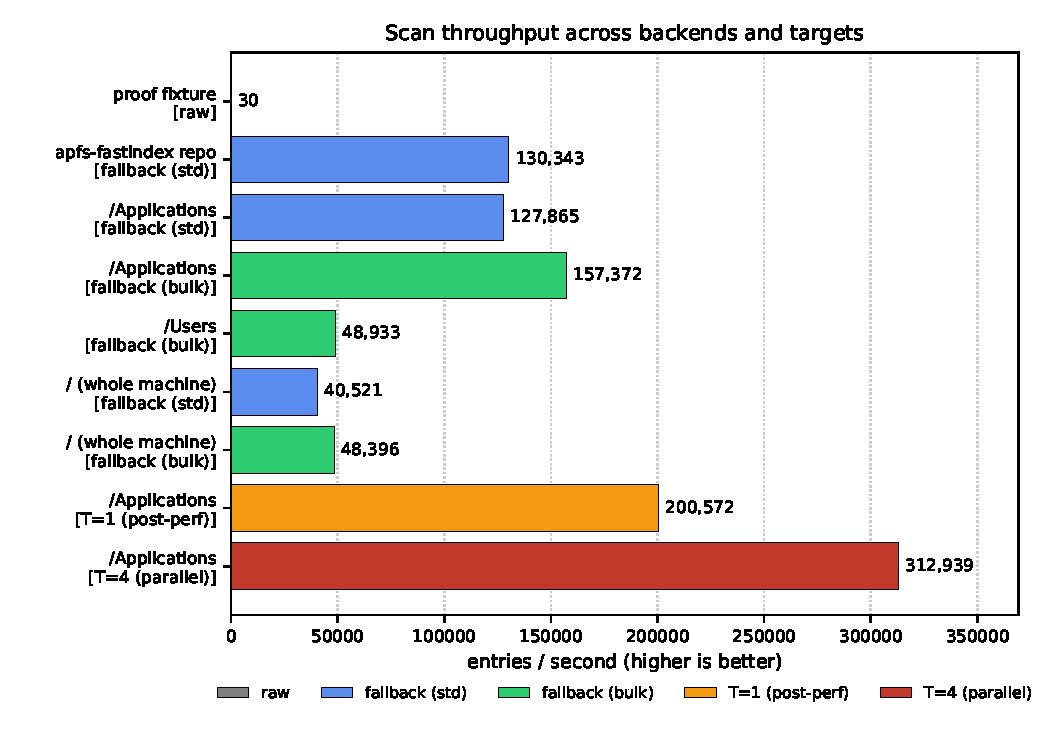
\includegraphics[width=\linewidth]{figures/perf-throughput.pdf}
\caption{Entries per second across the measurement rows. The proof
  fixture is dominated by \texttt{hdiutil attach} setup; the fallback
  rows cluster between forty and one-hundred-sixty thousand entries
  per second depending on backend and tree shape.}
\end{figure}

\begin{figure}[h]
\centering
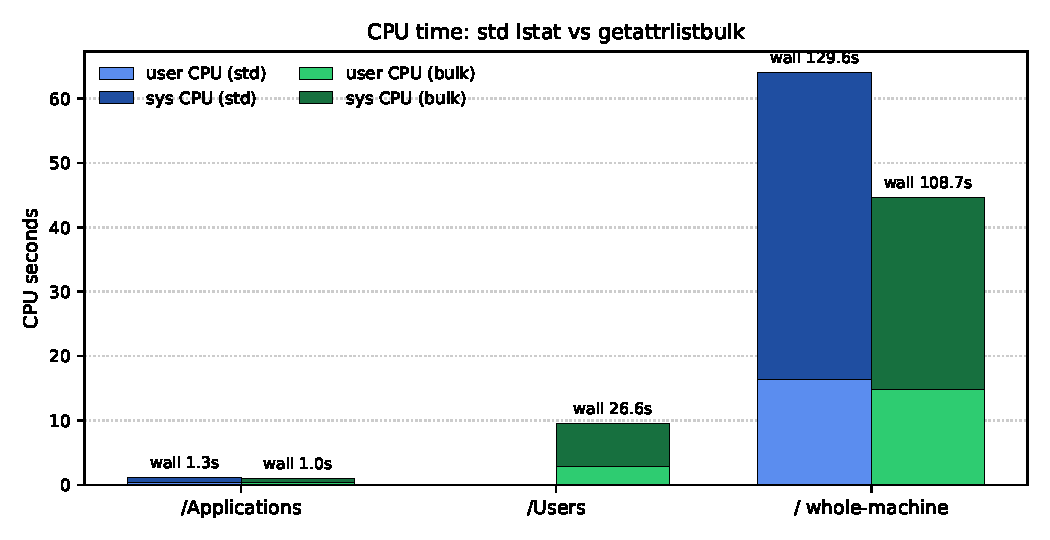
\includegraphics[width=\linewidth]{figures/perf-cpu.pdf}
\caption{User-plus-system CPU per row, comparing ordinary
  \texttt{lstat} against \texttt{getattrlistbulk}. The wall-time
  improvement is real but modest; the system-CPU drop is the cleaner
  signal that bulk fetch is doing less per-entry work in the kernel.}
\end{figure}

\section{Reading The Numbers}

\paragraph{The proof-fixture raw number is dominated by setup.}
Most of the 0.23 s is \texttt{hdiutil attach}; the actual seven-entry
walk is sub-millisecond. The raw-mode throughput on a meaningful
real volume is not yet measured because the project does not carry
a large detached APFS sample. The number above is honest but
unrepresentative.

\paragraph{Fallback throughput sits at roughly 130 thousand entries
per second on warm trees with \texttt{lstat} and roughly 157 thousand
with \texttt{getattrlistbulk}.} The improvement on \texttt{/Applications}
is about 24 per cent throughput. On the cold \texttt{/} scan the
improvement is smaller: 16 per cent wall, because the disk is the
bottleneck on a cold-cache run.

\paragraph{The cleaner perf signal is system CPU, not wall time.}
\texttt{getattrlistbulk} drops cold-\texttt{/} system CPU from 48 s
to 30 s, a 38 per cent reduction --- the kernel is doing
significantly less work per entry because batching cuts the
syscall count. The wall-time savings will compound on warm-cache
runs where the disk is not the constraint.

\paragraph{Symlinks remain at one extra \texttt{readlink} per entry.}
\texttt{getattrlistbulk} returns most file metadata in batch but does
not return link targets. The fallback walker fetches the target with
\texttt{readlink} when an entry is a symlink, which adds one
syscall per symlink. On filesystem trees with many symlinks (Python
virtualenvs, macOS frameworks) this is visible; on trees with few,
it is invisible.

\section{What The Numbers Do Not Say}

The table is a baseline; it is not a claim about anything beyond what
it measures. Three categories of question are explicitly outside the
table:

\begin{enumerate}
  \item Raw-mode throughput on a real source. The project has not
    measured raw mode on a representative live or detached volume
    of meaningful size. Until it does, the comparison "raw vs
    fallback" cannot be made.
  \item Incremental scans. The current model is full reparse on
    every run; the cache work of chapter~10 has not landed in
    product. Repeat-scan numbers will only mean something after a
    cache implementation passes its own oracle.
  \item Allocated, exclusive, or shared bytes. The R2-A lane in
    chapter~13 will change the cost model when it lands. The
    current numbers are for namespace plus logical size; adding
    extent-tree work will add measurement that the table does not
    capture.
\end{enumerate}

\section{The Measurement Discipline}

The discipline behind the table is what justifies leaning on it:

\paragraph{Measure before optimising.} The bulk-syscall improvement
was implemented after the standard \texttt{lstat} fallback was
measured, so the gain could be quantified. Optimisation without
measurement produces code whose effects nobody can describe.

\paragraph{Record the source class and the semantic mode with each
number.} The table above carries both. A throughput number without
those is not interpretable: 130 thousand entries per second is
either impressive or unimpressive depending on whether it ran on a
cold disk or a warm one, against raw or fallback, against
\texttt{/Applications} or \texttt{/}.

\paragraph{Hold the baseline.} Any future performance claim has to
compare against the table or against a row added to the table with
the same shape. A new optimisation that does not improve a baseline
row is not yet evidence of an improvement; it is a hypothesis
awaiting measurement.

The baseline above is conservative. The R2 work in chapter~13 will
have its own measurements, and the table will grow. The discipline
that keeps the table honest is the same discipline that keeps the
manual honest.
